\section{Introduction}
    Since the last document, some changes have been made to the project structure. The reward function has
    changed slightly, more environments were created/tested, the environment was made rotationally invariant,
    and training on a single start/goal position pair was made the focus.

\section{Reward Function}
    The reward function is mostly unchanged from what was written in the previous report. The main difference here
    is that a reward for flying in the direction of the goal was introduced. This new reward component is
    \begin{equation}
        r_{dir} = -C_3 S_C(\vec{v}_{goal}, \vec{a})
    \end{equation}
    where $C_3$ is a hyperparameter, $S_C$ is the cosine similarity between two vectors, $\vec{v}_{goal}$ is the
    vector from current position to the goal, and $\vec{a}$ is the action vector taken by the agent.

    The rest of the reward components mentioned in the previous paper are still present. I played with the weighting
    of each component, and also tried using both direction and distance reward components, only direction, and only
    distance, but wasn't able to see appreciable different between each. One downside of the direction goal component
    is that the agent may learn to draw out episodes to continue receiving more reward. The weighting of the reward
    components must be tuned to prevent this.

\section{New Environments}
    Some new environments were made to perform testing and training. The training environment was made to be simple
    with very simple obstacles in order to test generalization performance of the trained agent. For testing, a map
    of the buildings of Ohio University's West Green was made. These environments can be found in the following figure.

    \begin{figure}[H]
        \centering
            
\includegraphics[width=2.75cm,frame]{grid_general2.png}
            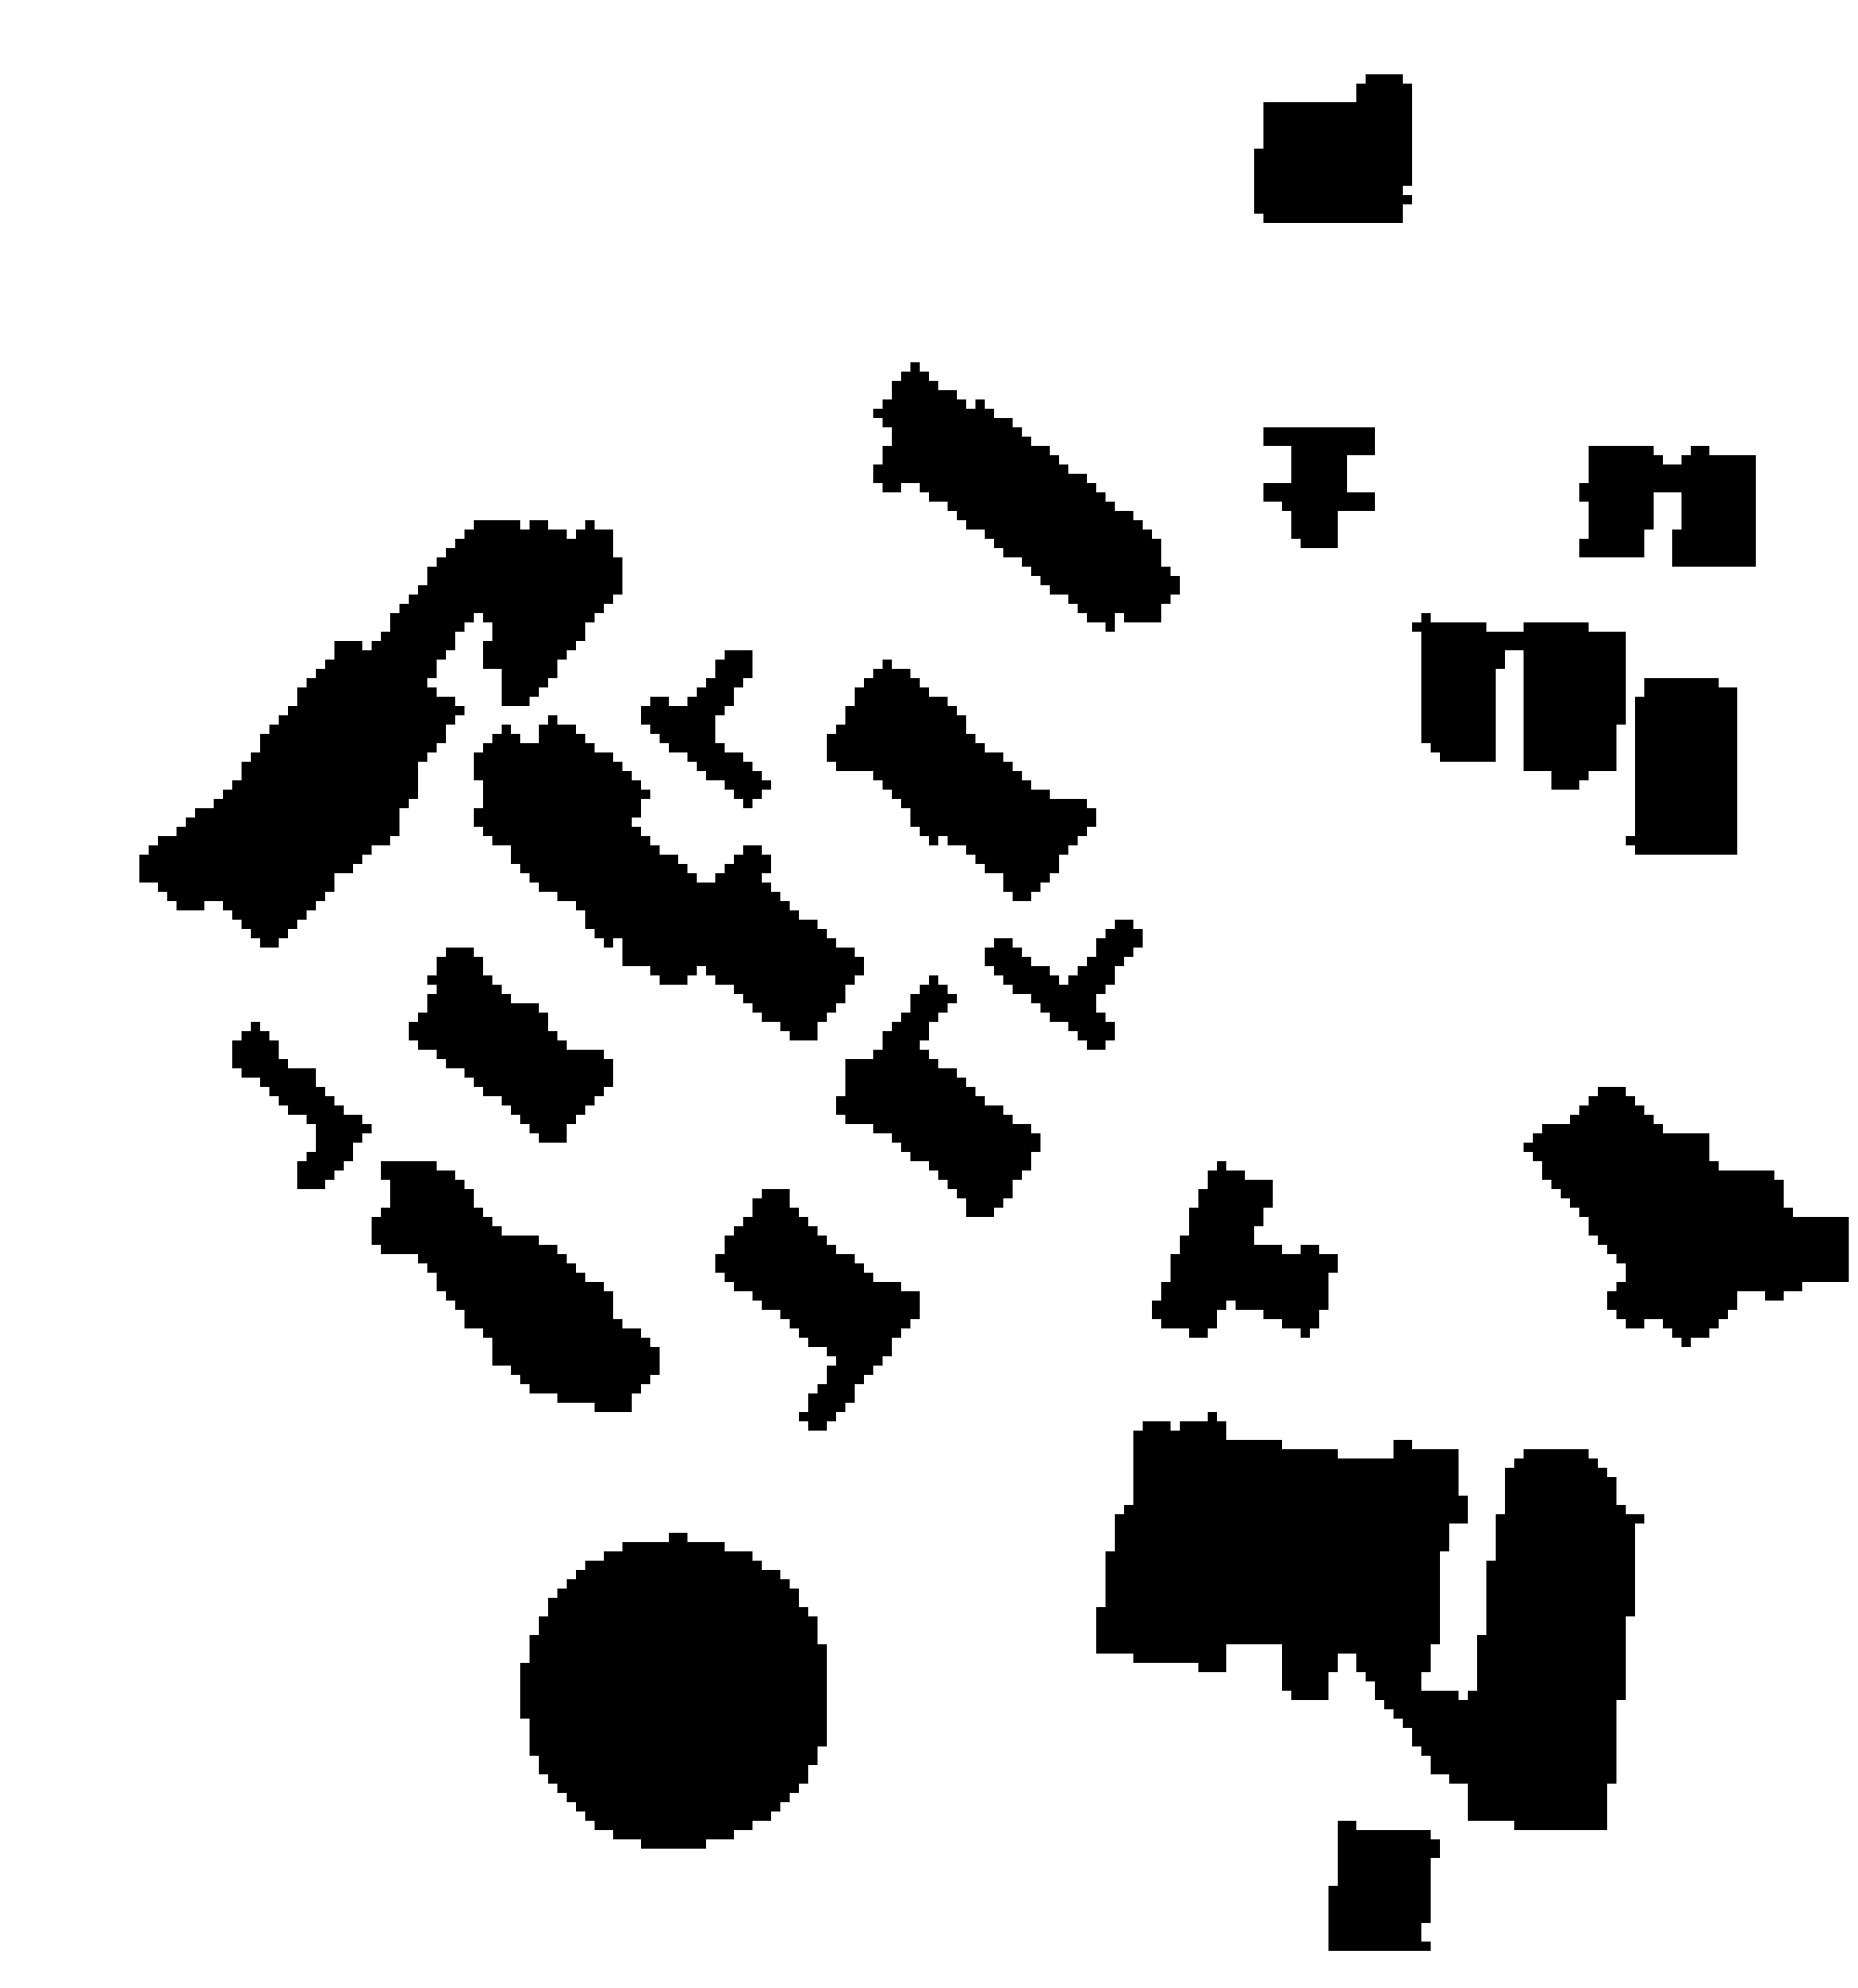
\includegraphics[width=2.75cm,frame]{west_green_small.png}
            \caption{New environments for training and testing. Left is simple training env, right is Ohio University's
                     West Green, used for testing.}
            \label{fig:environments}
    \end{figure}

\section{Rotational Invariance}
    In order to best support generalization performance of the trained agent, the environment was made with rotational
    invariance in mind. In essence, this means that when the start/goal positions are set, the orientation of the
    environment is locked. The axis of rotation is set to the directional vector from the start position to the goal position.
    Then, all directional vectors (actions, observation vectors, etc.) are relative to this rotation axis. For example, the
    vector $(0, 1)$ represents the unit vector pointing from the start position to the goal position. This rotational axis does
    not change within an episode.

    The idea for this mechanism is that the agent generally learns to move towards the goal, only turning if an obstacle warrants
    it. Then, when moving to a different start/goal position pair or a new environment entirely, the rotational invariance ensures
    that the learned policy is transferable. The agent should still understand how to move towards the goal.

\section{Single Start/Goal Pair}
    Changed from the last report is also the process of training of a single start/goal position pair. Previously, training was
    done on random start/goal pairs. This was done to encourage a robust learned policy that could adapt to many environments. However,
    due to differences in the total reward based on different start/end pairs, this introduced too much variance in the training process,
    leading to unstable training. Hence, training for a single start/end pair seems more appropriate.

\section{Results}
    Unfortunately, I could not achieve good results, even with the changes listed in this document. The training process is not
    stable and often results in a policy that prefers making the action vector $(1, 1)$ or $(-1, 1)$. I believe this may ultimately
    be due to a mistake in my training/environment setup or simply a bug in my DDPG implementation.

\section{Future Considerations}
    If a researcher in the future wants to explore DRL for path planning, I would advise writing the implementation in PyTorch rather
    than TensorFlow. Prior to writing this project, I was more comfortable with TensorFlow, but I have since found that PyTorch is more
    flexible and more widely used in research contexts. Especially for DRL applications where training loops are implemented by hand,
    PyTorch's design model seems more appropriate.

    Furthermore, a redesign of the environment may be useful. Currently, the main problem with training was that the learned policy would
    choose the actions $(1, 1)$ and $(-1, 1)$. I believe this may be related to instabilities in the training process causing the gradients
    to explode and then get "stuck" at the extremes due to gradient squashing with the tanh activation function. It may be more appropriate
    to make the agent choose actions as angle and magnitude rather than euclidean direction vectors. This encoding may avoid some of the
    problems I experienced.
    
    Also, the local window view of the environment as input to the model may not be the most effective for the path planning
    problem. In my experience with a previous project (and other researcher's results), LIDAR data may be a better alternative.
    With LIDAR, the agent has the ability to see obstacles further away than with the local window approach. Also, since LIDAR data
    is already encoded as distance from the agent, I believe it's conceptually more useful or more easily trainable than the local
    window approach.

    Finally, I believe DDPG may not be the best DRL algorithm for this task. I tried TD3 briefly, but didn't see much difference. More exploration
    could be done here.

    In all, I believe the project has potential, but it needs a lot of big redesigns. My advice for any future researchers is to use my code
    as a reference while writing your own new implementation in PyTorch.